\chapter*{Introduction}
\label{introduction}
%
The goal of this paper is to analyse results from a study called \textit{Men and Bread} using Principal Component Analysis (PCA). \blankline
% 
In the study \textit{Men and Bread} 21 subject was asked to rated different types of buns according to different attributes. Eight different types of buns and one other type of bun for familiarization, were presented to the subjects for rating. The buns presented in the study is shown in \autoref{fig:bread}, where bread B9 was used for familiarization. 
%
\begin{figure}[H]
\centering
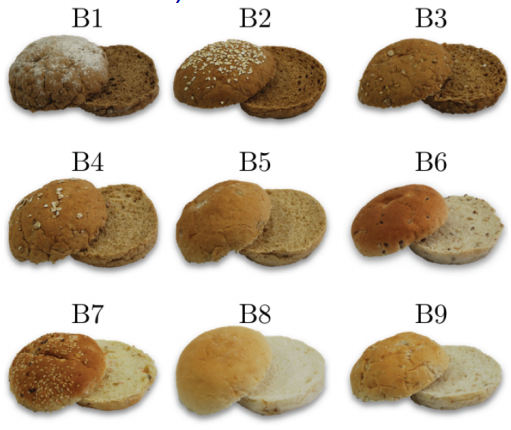
\includegraphics[width =0.7\textwidth]{Figure/Bread}
\caption{The different types of buns with identifying name, presented so that both crust and crumb can be seen.}
\label{fig:bread}
\end{figure}
\noindent
%
For each one of the different types of buns 11 different attributes from three different groups were rated. 


\begin{tabular}{ |l|l| }
\hline
\multicolumn{2}{ |c| }{\textbf{Reflection}} \\
\hline
\textit{Attribute} & \textit{Scale Question} \\ 
\hline
\multirow{2}{*}{Filling} & Hvor mættende ser brødet ud? (lidt til meget) \\
 &  How filling is the bread? (a little to a lot) \\ \hline
\multirow{2}{*}{Nourishing} & Hvor nærende ser brødet ud? (usundt til sundt) \\
 &   How nourishing is the bread? (healthy to unhealthy) \\ \hline
\multirow{2}{*}{Wholegrain} & Hvor fuldkornsholdigt er brødet? (lidt til meget) \\
 &   How large is the amount of wholegrain in the bread? (low to high) \\ \hline
\multirow{2}{*}{Fibre} & Hvor fiberholdigt er brødet? (lidt til meget) \\ 
 &   How fibrous is the bread? (low to high))\\ 
\hline
\end{tabular}



The buns were rated on Visual Analog Scale (VAS) with open endpoints. An example of the scale is shown in \autoref{fig:Skala}. 
%
\begin{figure}[H]
\centering
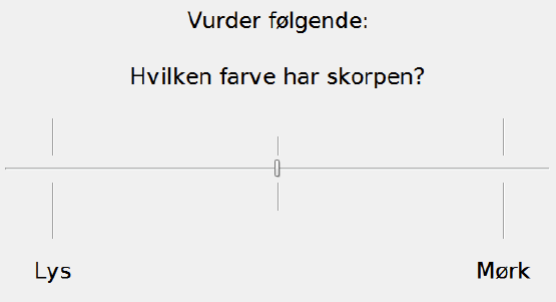
\includegraphics[width =0.7\textwidth]{Figure/Skala}
\caption{Example of the VAS scale used in the study \textit{Men and Bread}.}
\label{fig:Skala}
\end{figure}
\noindent



%Analyze the results from the example using PCA.

%First plot a “profile” of all stimuli.

%How much of the variance is explained by each component?

%(Plot a scree-plot including cumulative variance).

%Plot your PCA solution graphically. Both a plot with just your stimuli (scores) and a biplot with both scores and loadings.

%Make a table of the loadings of each word-pair on each principal component.

%Interpret the solution. Also, are there word-pairs that seem ”redundant” e.g. measures that same perceptual attribute?
